
\section{Questions de recherche}


\begin{figure}
  \begin{center}
    
\begin{tikzpicture}[scale=1.2]

  \newcommand\X{125pt}
  \newcommand\Y{100pt}
  
  \newcommand\LIGHTGRAY{gray!20}
  \newcommand\MEDIUMGRAY{gray!40}
  
  \draw(0,0) +(-\X, -\Y) rectangle +( \X, \Y);
  
  \draw[fill=\LIGHTGRAY](-0.5*\X,-0.5*\Y) +(-0.5*\X,-0.5*\Y) rectangle +(0.5*\X,0.5*\Y);
  \draw(-0.5*\X, 0.5*\Y) +(-0.5*\X,-0.5*\Y) rectangle +(0.5*\X,0.5*\Y);
  \draw(0.5*\X,-0.5*\Y) +(-0.5*\X,-0.5*\Y) rectangle +(0.5*\X,0.5*\Y);
  \draw[fill=\LIGHTGRAY](0.5*\X, 0.5*\Y) +(-0.5*\X,-0.5*\Y) rectangle +(0.5*\X,0.5*\Y);
  
  \draw(-0.5*\X,\Y) node[anchor=south]{\textsc{same time}};
  \draw(0.5*\X,\Y) node[anchor=south]{\textsc{different time}};
  \draw(-\X,0.5*\Y) node[anchor=east]{\textsc{same place}};
  \draw(-\X,-0.5*\Y) node[anchor=east]{\textsc{different place}};

  \small

  \draw (-0.5*\X, 0.5*\Y) node[align=center]{\textbf{Face to face interactions}\\
    (e.g. decision rooms, single\\ display groupware, shared\\ table, wall displays,
    roomware)};

  \draw ( 0.5*\X, 0.5*\Y) node[align=center]{\textbf{Continuous task}\\ (e.g. team rooms,
    large public\\ displays, shift work, groupware,\\ project management)};

  \draw (-0.5*\X,-0.5*\Y) node[align=center]{\DARKBLUE{\textbf{Remote
        interactions}}\\
    (e.g. video,
    conferencing,\\ instant messaging,\\ chats/MUDs/virtual worlds,\\ shared screens,
    multi-user\\ editors)};

  \draw ( 0.5*\X,-0.5*\Y) node[align=center]{
    \textbf{Communication + coordination}\\
    (e.g. email, bulletin boards,\\ blogs, asynchronous\\ conferencing, group
    calendars,\\ workflow, version control,\\ wikis)};

\end{tikzpicture}
    \caption[Matrice de répartition des systèmes collaboratifs] {
      \label{editor:fig:groupware} Matrice de répartition des systèmes
      collaboratifs~\cite{johansen1988groupware}.}
  \end{center}
\end{figure}

L'édition collaborative répartit l'écriture selon deux dimensions : le temps et
l'espace~\cite{desanctis1987foundation, grudin1994computersupported,
  johansen1988groupware}.  La figure~\ref{editor:fig:groupware} résume cette
répartition. Dans ce manuscrit, nous nous intéressons particulièrement aux
collaborateurs connectés en même temps en des lieux différents correspondant à
la problématique du temps réel. Dans ce contexte, \og temps réel \fg signifie
que les modifications doivent être perçues au plus
tôt~\cite{ellis1989concurrency}. La tolérance d'un utilisateur varie selon les
outils collaboratifs à sa disposition. Une modification locale doit être
observée immédiatement. En revanche, une modification distante est plus lente à
être observée.

\begin{figure}
  \begin{center}
    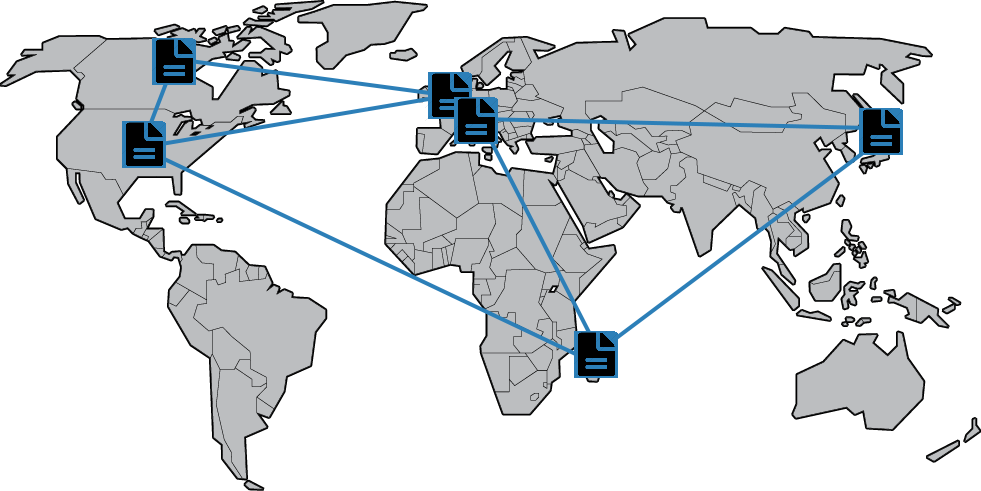
\includegraphics[width=0.85\textwidth]{img/world.png}
    \caption[Édition collaborative décentralisée]{\label{intro:img:world}Édition
      collaborative décentralisée répartie à travers le monde.}
  \end{center}
\end{figure}

Un éditeur de texte tel que Microsoft Word~\cite{word} ou Emacs~\cite{emacs}
permet à un utilisateur de créer et d'éditer un document. Un éditeur de texte
collaboratif temps réel~\cite{ellis1991groupware} étend la rédaction d'un
document à un groupe d'utilisateurs potentiellement distants les uns des autres.
Par exemple, la figure~\ref{intro:img:world} présente une session d'édition
comprenant 6 instances d'un même éditeur collaboratif réparties à travers le
monde éditant un même document. Chacun possède son éditeur, voit les
modifications effectuées par ses collaborateurs sur le document, effectue ses
propres changements en insérant ou en supprimant du contenu.  La mise en place
de ces fonctionnalités temps réel requiert
\begin{inparaenum}[(i)]
\item un moyen de représenter les documents en mémoire de telle sorte que tous
  les éditeurs affichent un même document lorsqu'ils ont reçu les mêmes
  modifications~\cite{burckhardt2014replicated, shapiro2011conflict};
\item un moyen de communication fiable entre les éditeurs fonctionnant sur des
  machines potentiellement distantes.
\end{inparaenum}

Afin d'augmenter la disponibilité du document et de diminuer le temps de réponse
lors d'une modification, les éditeurs collaboratifs actuels suivent le principe
de la réplication optimiste~\cite{saito2005optimistic}. Chaque éditeur
collaboratif possède une copie locale d'un document -- pouvant être représenté
simplement par une séquence
%\footnote{ou liste, ou tableau, ou série.} 
de caractères autorisant les deux opérations suivantes :
\begin{inparaenum}[(a)]
\item l'insertion d'un caractère à une position dans la séquence et
\item la suppression du caractère à une position dans la séquence.
\end{inparaenum}
Lorsque l'utilisateur effectue une opération
\begin{inparaenum}[(i)]
\item elle est directement répercutée sur sa copie avant
\item d'être envoyée au reste des éditeurs où
\item elle est intégrée.
\end{inparaenum}
Les séquences répliquées convergent vers un état identique sous l'hypothèse
d'une diffusion fiable des opérations, i.e., tous les éditeurs reçoivent toutes
les modifications.

Pour assurer la convergence des répliques, l'utilisation des structures de
données \og classiques \fg n'est pas directement possible. % du fait de la latence
%entre les collaborateurs.
Par exemple, la figure~\ref{intro:fig:ripconvergence} présente une situation où
un auteur insère un caractère sur la réplique 1 en début de document pendant
qu'un autre supprime un caractère sur la réplique 3 au même endroit. Le premier
auteur voit le caractère qu'il vient d'insérer supprimé. Quant à l'état final de
la réplique 2, il dépend de l'ordre de réception des opérations. Ici, la
suppression arrivant avant l'insertion, la séquence répliquée devient
\texttt{QERTY}.  Afin d'éviter de telles divergences dans l'état des répliques,
de nouvelles structures et de nouveaux algorithmes adaptés au contexte réparti
doivent être employés.


\begin{figure}
  
\begin{tikzpicture}[scale=1.2]

  \newcommand\X{30pt};
  \newcommand\Y{30pt};
  
  \draw[->](0pt,   0pt)--(10*\X,   0pt);
  \draw[->](0pt, -1*\Y)--(10*\X, -1*\Y);
  \draw[->](0pt, -2*\Y)--(10*\X, -2*\Y);
  
  \draw[fill=black](0pt, 0pt) node[anchor=east]{réplique 1 }circle(2pt);
  \draw[fill=black](0pt, -1*\Y) node[anchor=east]{réplique 2 }circle(2pt);
  \draw[fill=black](0pt, -2*\Y) node[anchor=east]{réplique 3 }circle(2pt);

  \draw(\X,2pt)--node[anchor=south]{[WERTY]}( \X,   -2pt);
  \draw(\X,2 -1*\Y)--node[anchor=south]{[WERTY]}(\X,-2 -1*\Y);
  \draw(\X,2 -2*\Y)--node[anchor=south]{[WERTY]}(\X,-2 -2*\Y);
  \small
  \draw(3* \X,2pt)--node[anchor=north]{\textsc{insert}(\DARKBLUE{Q, 0})}(3 * \X,   -2pt);
  \draw(3* \X,2 -2*\Y)--node[anchor=north]{\textsc{delete}(\DARKBLUE{\textbf{0}})}(3 * \X,-2 -2*\Y);
  \normalsize

  \draw(3* \X,2pt)--node[anchor=south]{[QWERTY]}(3 * \X,   -2pt);
%  \draw(2* \X,2 -1*\Y)--node[anchor=south]{[ ]}(2* \X,-2 -1*\Y)
  \draw(3* \X,2 -2*\Y)--node[anchor=south]{[ERTY]}( 3 * \X,-2 -2*\Y);

  \draw[->, dashed] (5*\X, 0pt) -- (15+7*\X, -1*\Y);
  \draw[->, dashed] (5*\X, 0pt) -- (7*\X, -2*\Y);

  \small
  \draw[->, dashed] (5*\X, -2*\Y) -- (7*\X,  0*\Y)
  node[anchor=south]{\textsc{delete}(\DARKBLUE{\textbf{0}})};
  \normalsize
  \draw[->, dashed] (5*\X, -2*\Y) -- (7*\X, -1*\Y);

  \draw(9*\X, 2 -0*\Y)--node[anchor=south]{[WERTY]}(9*\X,-2 -0*\Y);
  \draw(9*\X, 2 -1*\Y)--node[anchor=south]{[QERTY]}(9*\X,-2 -1*\Y);
  \draw(9*\X, 2 -2*\Y)--node[anchor=south]{[QERTY]}(9*\X,-2 -2*\Y);


%%  \draw(9*\X, 2 -0*\Y)--node[anchor=south]{[QWERTY]}(9*\X,-2 -0*\Y);
%%  \draw(9*\X, 2 -1*\Y)--node[anchor=south]{[QWERTY]}(9*\X,-2 -1*\Y);
%%  \draw(9*\X, 2 -2*\Y)--node[anchor=south]{[QWERTY]}(9*\X,-2 -2*\Y);


%%  \draw[fill=white, very thick]
%%  (0*\X, 0*\Y) node{$p_1$} +(-5pt,-5pt) rectangle +(5pt,5pt);
%%  \draw[->](-5+\X, 5+2*\Y)to[out=120,in=30](0pt,5+2*\Y); %% 6 -> 7
\end{tikzpicture}
  \caption{\label{intro:fig:ripconvergence} Répliques divergentes d'un
    document.}
\end{figure}


Une première famille d'approches consiste à transformer les arguments de toute
opération afin qu'elle considère les opérations intégrées
concurremment~\cite{sun1998operational}. Dans l'exemple précédent, lors de
l'intégration de la suppression par le premier éditeur, celui-ci doit réaliser
qu'un caractère a été ajouté en tête concurremment. Il doit donc modifier les
arguments de l'opération reçue afin que le caractère \texttt{W} soit supprimé,
et non plus le caractère \texttt{Q}. Toutes les répliques convergent alors vers
la séquence \texttt{QERTY}.  Détecter ces cas concurrents nécessite de
communiquer, avec chaque opération, des données dont la croissance est
linéaire~\cite{charronbost1991concerning, sun2009contextbased}. Cette contrainte
confine l'emploi de ces approches aux petits groupes d'utilisateurs.

Une seconde famille d'approches consiste à utiliser des structures de données
dont les opérations sont commutatives~\cite{shapiro2011conflict} et ne souffrent
donc pas de la concurrence. Pour que les opérations commutent, ces approches
associent à chaque caractère de la séquence un identifiant unique et
immuable. Nous distinguons deux types de structures se différenciant par la
nature des identifiants considérés :

\paragraph{Les identifiants cachés~\cite{oster2006data}.} L'opération de
suppression de caractères se contente de cacher le caractère ciblé par
l'utilisateur. La mémoire consommée par une réplique croît de manière monotone
par rapport au nombre d'insertions.
% Les performances d'intégration des opérations s'en trouvent diminuées.
La structure répliquée d'un document vide peut contenir des milliers
d'identifiants cachés correspondant à des caractères supprimés.  Afin d'y
remédier, un protocole de ramasse-miettes réparti~\cite{abdullahi1998garbage}
doit être exécuté régulièrement pour purger la structure des identifiants
cachés. Malheureusement, cela s'avère extrêmement
coûteux~\cite{abdullahi1998garbage}.

\paragraph{Les identifiants de taille variable~\cite{weiss2009logoot}.} Les
identifiants sont des listes dont la taille est fixée à la
génération. Cependant, la fonction de génération d'identifiants alloue des
identifiants dont la taille peut dépendre linéairement du nombre d'insertions
dans la séquence~\cite{weiss2009logoot}.
% Cette croissance impacte négativement les performances du système.
Puisque chaque identifiant doit être envoyé à toutes les autres répliques, le
trafic généré peut augmenter rapidement.  Afin d'y remédier, un protocole de
relocalisation des identifiants doit être exécuté
régulièrement~\cite{zawirskiasynchronous}. Ces protocoles reviennent à obtenir
un consensus dans un contexte réparti. Malheureusement, cela s'avère extrêmement
coûteux~\cite{mostefaoui2015signature}.

Cela pose la première question de recherche : \textbf{Afin d'éviter tout
  protocole additionnel de relocalisation des identifiants, comment allouer ces
  identifiants de sorte que leur taille soit directement sous-linéaire ?}

Afin d'assurer la convergence de toutes les répliques du document vers un état
équivalent, les éditeurs collaboratifs font l'hypothèse d'une communication
fiable : chacune des modifications doit être reçue par l'ensemble des éditeurs
collaboratifs.
%%Pour converger vers des documents identiques, tous les changements doivent
%% parvenir à tous les éditeurs.
Une manière efficace de mettre en place cette diffusion fiable et décentralisée
consiste à suivre le principe de dissémination épidémique\footnote{ou propagation
  de rumeurs.}  où
\begin{inparaenum}[(i)]
\item l'éditeur effectuant un changement choisit un sous-ensemble d'éditeurs
  possédant une réplique du document et leur envoie la modification;
\item lorsqu'un éditeur reçoit un tel message, il choisit à son tour un
  sous-ensemble d'éditeurs auxquels faire suivre le message.
\end{inparaenum}
Les changements atteignent tous les éditeurs par transitivité.
% Par conséquent, un réseau superposé doit être mis en place afin de permettre une
% communication fiable d'un éditeur à l'autre.
La figure~\ref{intro:img:world} montre que chaque éditeur collaboratif est
connecté à d'autres éditeurs -- ses voisins -- possédant une réplique du
document. Ici, l'éditeur localisé aux États-Unis communique avec les éditeurs
canadien, français et malgache.
% Chaque éditeur participe activement au bon fonctionnement
%du système.
Une opération émise par ce premier peut transiter par l'éditeur localisé à
Madagascar avant de parvenir à l'éditeur japonais. 
% Les changements parviennent
%à tous les éditeurs par transitivité~\cite{birman1999bimodal}.

\noindent Notre contexte nous expose à deux contraintes :

\begin{enumerate}[(i)]
%\paragraph{Web.}
\item L'éditeur collaboratif doit fonctionner dans les navigateurs Web sans
  installations d'aucune sorte (e.g. extensions). Depuis peu, les navigateurs
  sont capables communiquer entre eux après avoir suivi un processus de
  connexion complexe~\cite{webrtc}. L'éditeur doit supporter ce mode de
  connexion.

%\paragraph{Dimensions et dynamisme.}
\item L'éditeur collaboratif doit maintenir un voisinage dont la taille gère
  aussi bien les petits groupes que les grands.  La taille des voisinages est
  déterminante puisque lorsqu'elle augmente, le trafic généré augmente au risque
  de dépasser les capacités d'émission des éditeurs; lorsqu'elle diminue,
%% les changements risquent de ne plus parvenir à tous les éditeurs.
  le risque que les opérations ne parviennent plus à tous les éditeurs augmente.
  L'éditeur doit supporter les sessions d'édition où le nombre de participants
  fluctue fortement au cours du temps.
\end{enumerate}

Les protocoles d'échantillonnage aléatoire de pairs~\cite{jelasity2007gossip}
permettent à chaque éditeur de peupler son voisinage d'éditeurs choisis
aléatoirement parmi les éditeurs impliqués dans la rédaction du document. Entre
autres, ces protocoles assurent une forte résilience aux arrivées et aux départs
dans la session collaborative -- comportement fréquent dans le contexte
Web. Cependant, la grande majorité de ces protocoles fournissent des voisinages
configurés \emph{a priori}, et donc, de taille
constante~\cite{eugster2003lightweight, jelasity2007gossip,
  leitao2007dependable, tolgyeski2009adaptive, voulgaris2005cyclon}. En d'autres
termes, le développeur doit connaître le nombre de participants impliqués dans
la rédaction d'un document afin de configurer la taille des voisinages
idéalement~\cite{erdos1959random}.  Pour ne pas renoncer aux grands groupes, les
voisinages doivent être surdimensionnés. Le trafic en résultant est élevé. Le
seul protocole permettant d'adapter automatiquement la taille des voisinages à
la taille de la session d'édition se nomme
\SCAMP~\cite{ganesh2003peer}. Toutefois, ce dernier est inadapté au processus
complexe d'établissement de connexions disponible dans les navigateurs Web.

% Malheureusement, celui-ci varie, que ce soit
%pendant la durée de la collaboration, e.g., un cours de formation en ligne
%(\emph{MOOC})~\cite{breslow2013studying} voit sa population fluctuer selon
%l'intérêt qu'il suscite; ou entre deux documents, e.g., un document créé pour un
%événement de grande ampleur n'a pas la même audience que celle d'un rapport de
%projet écrit par des étudiants.

Cela pose la seconde question de recherche : \textbf{Comment adapter
  efficacement le voisinage de chaque éditeur collaboratif Web au nombre
  fluctuant de collaborateurs ?}


%%% Local Variables:
%%% mode: latex
%%% TeX-master: "../../paper"
%%% End:
